
\subsection{2.14.  Диаграммы МО для галогенидов 15-ой – 18-ой групп.} 

\par\bigskip
 
 \begin{figure}[H]
 	\centering
 	{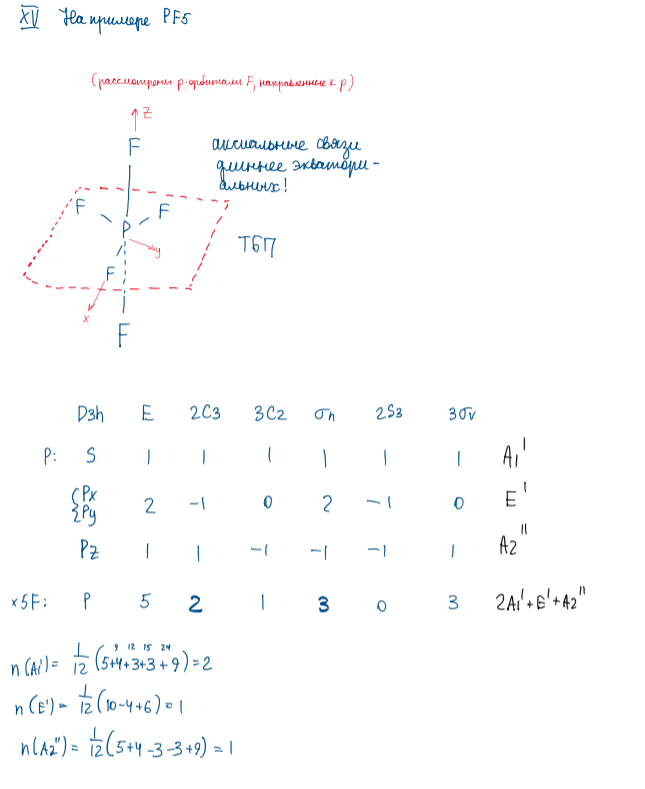
\includegraphics[scale=0.7]{74.png}}
 \end{figure}

\begin{figure}[H]
	\centering
	{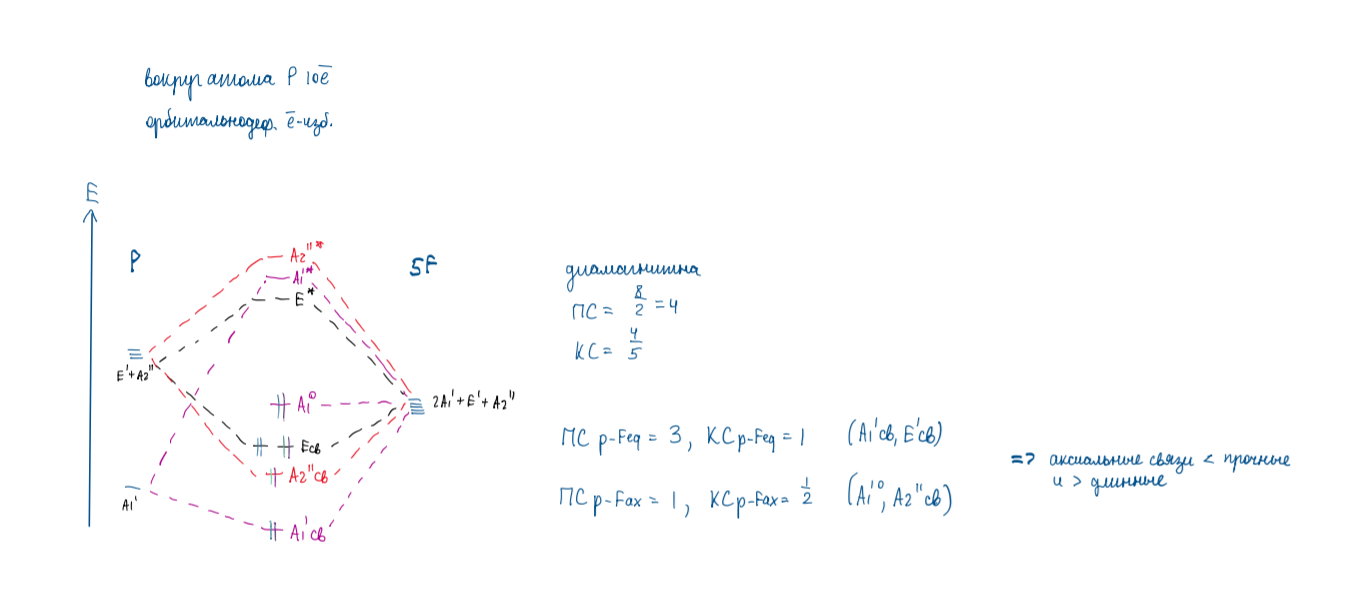
\includegraphics[scale=0.6]{75.png}}
\end{figure}
\begin{figure}[H]
	\centering
	{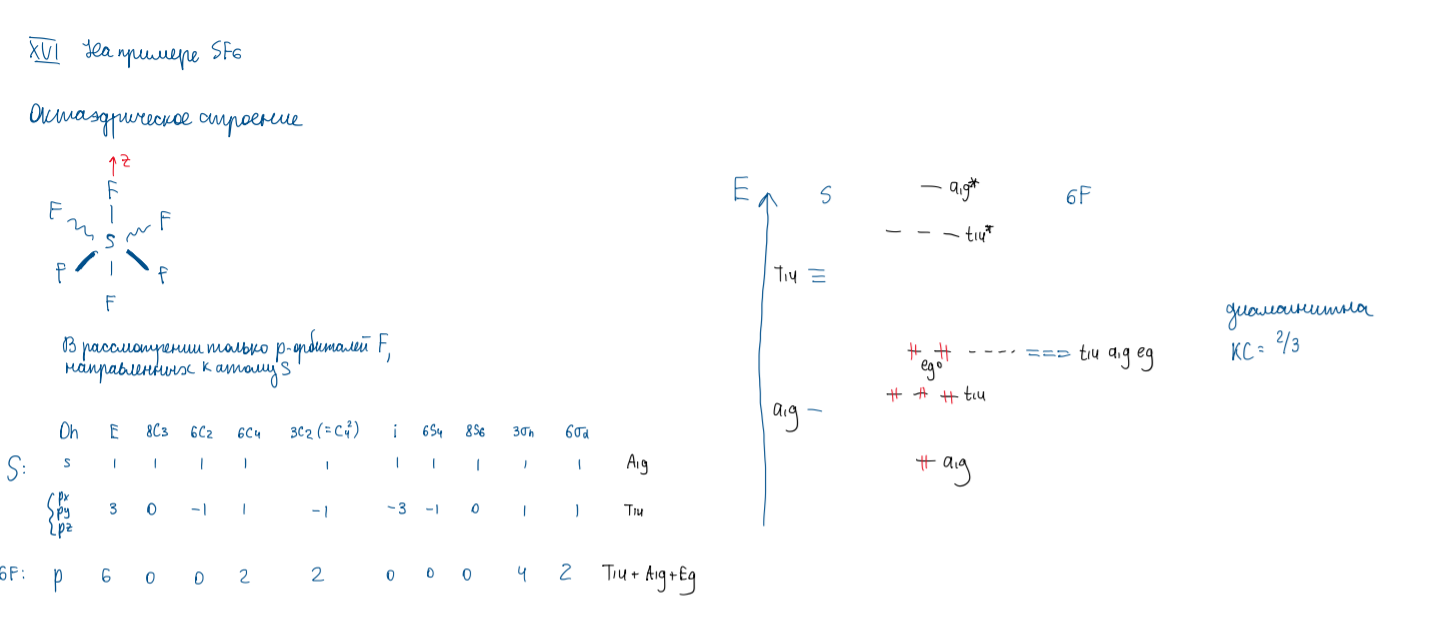
\includegraphics[scale=0.6]{76.png}}
\end{figure}
\begin{figure}[H]
	\centering
	{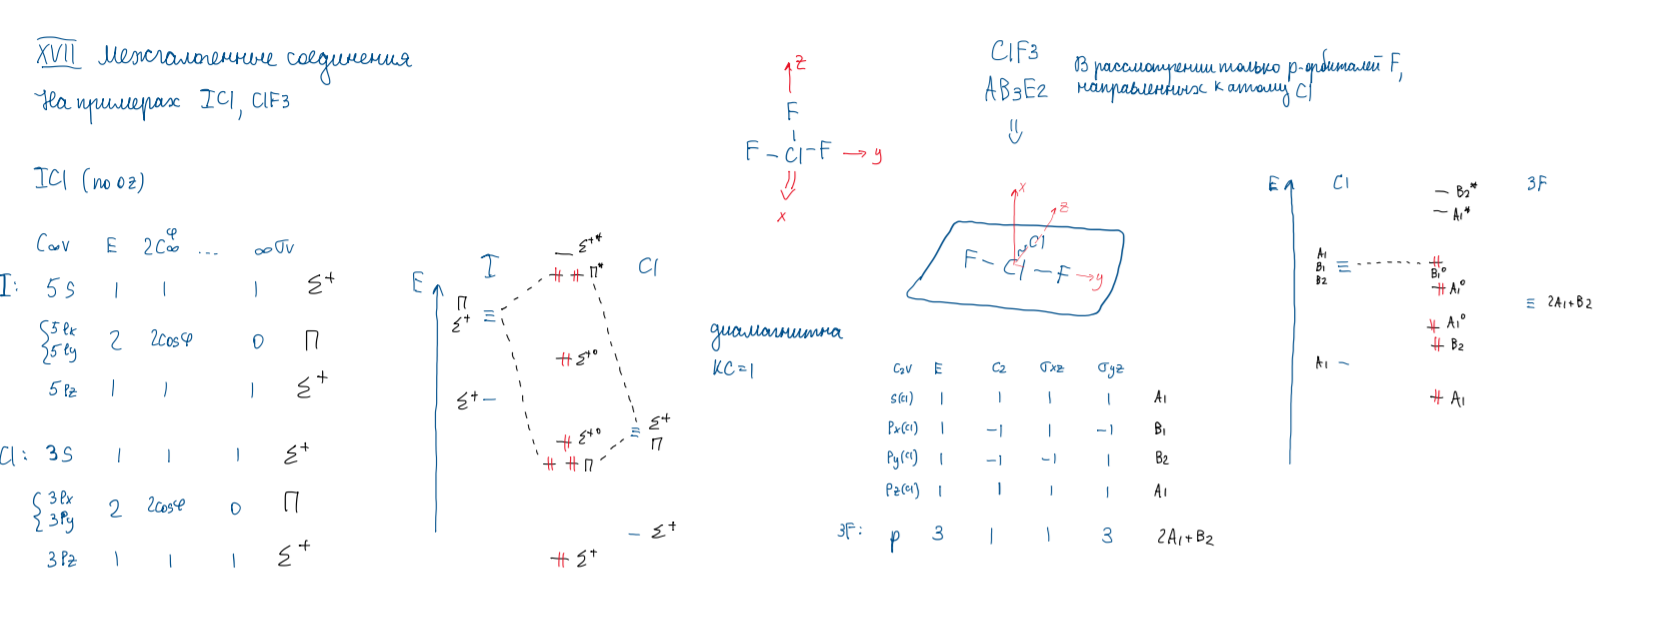
\includegraphics[scale=0.5]{77.png}}
\end{figure}
\begin{figure}[H]
	\centering
	{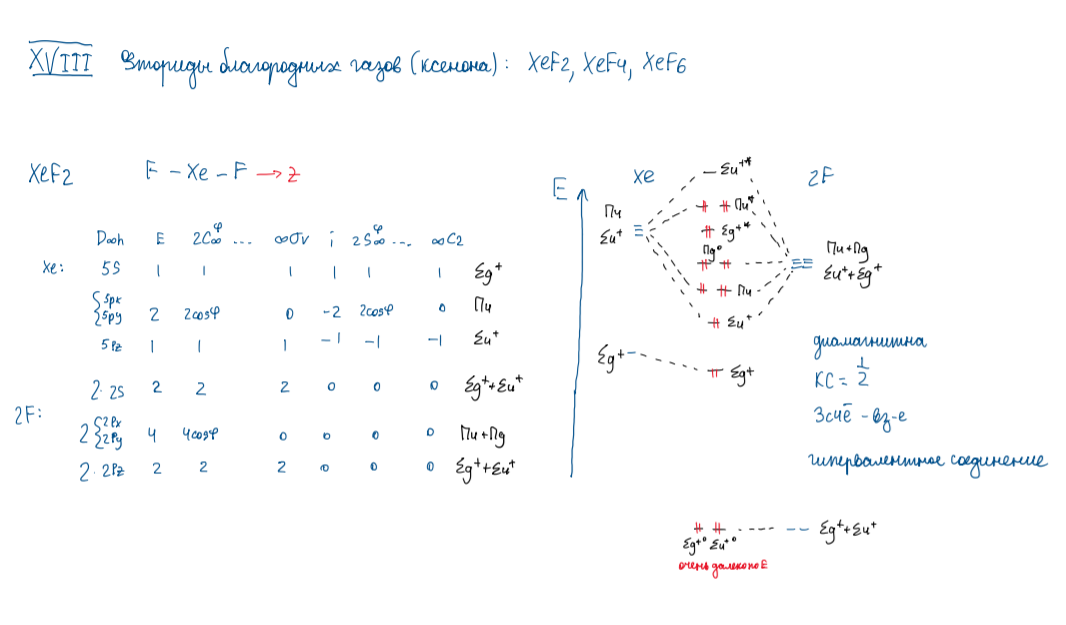
\includegraphics[scale=0.7]{78.png}}
\end{figure}
\begin{figure}[H]
	\centering
	{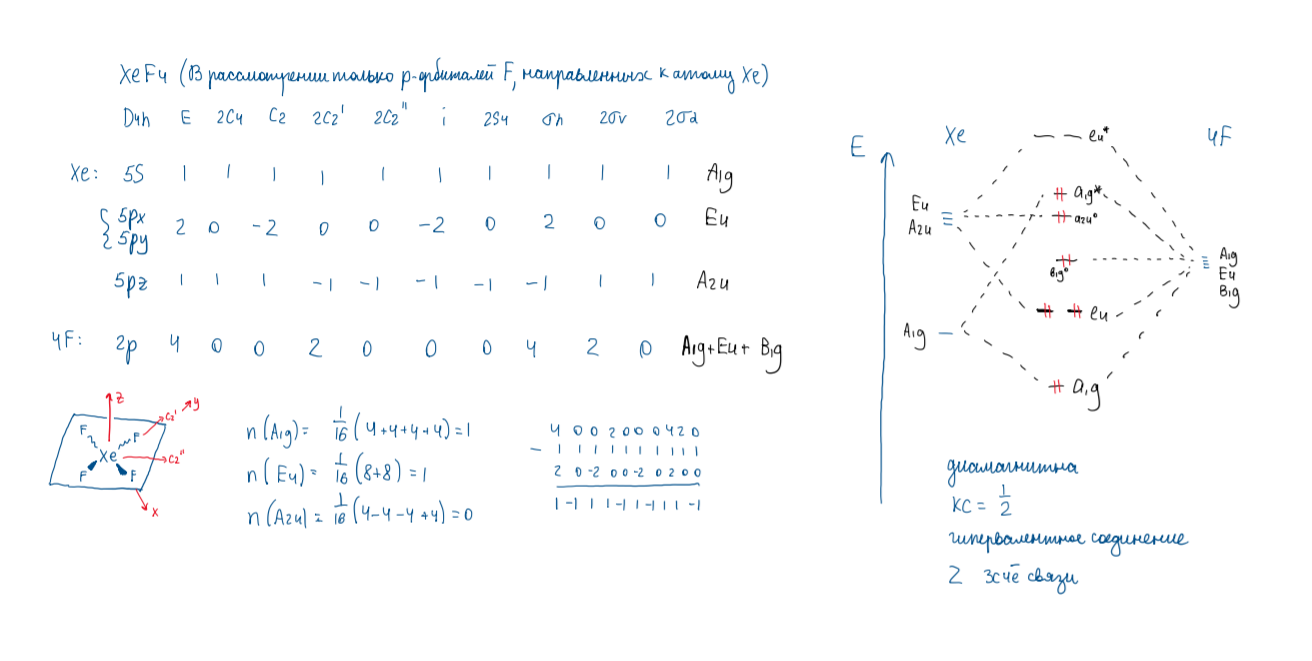
\includegraphics[scale=0.65]{79.png}}
\end{figure}
\begin{figure}[H]
	\centering
	{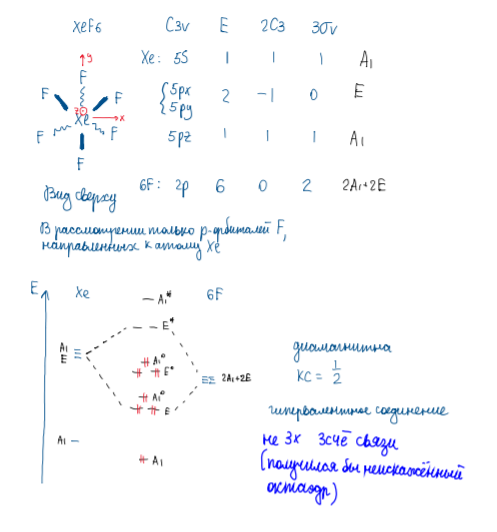
\includegraphics[scale=1]{80.png}}
\end{figure}
 	